\begin{frame}{Diseño e implementación de modelos.\newline Modelo de capas LSTM I}
	\vspace*{10pt}
	\normalsize{\underline{\textbf{Tipos de arquitectura}}}
	\vspace*{3pt}
	\begin{itemize}
		\scriptsize
		\item \textbf{One to one}\arrowTikz{0}clasificación de imágenes, una entrada (matriz de la imagen), una salida, la categoría.
		\item \textbf{One to many}\arrowTikz{0}generación de títulos para imágenes, una entrada (matriz de la imagen), varias salidas, las diferentes palabras.
		\item \textbf{Many to one}\arrowTikz{0}análisis de sentimiento, entran varias palabras, se clasifica como positiva o negativa.
		\item \textbf{Many to many}\arrowTikz{0}traducción de texto, varias palabras en un idioma a la entrada y varias a la salida en otro idioma.
		\item \textbf{Many to many}\arrowTikz{0}entradas y salidas sincronizadas, clasificación de vídeo.
	\end{itemize}
	\vspace*{-10pt}
	\begin{figure}[ht!]
		\centering
		\resizebox{\textwidth}{!}{
			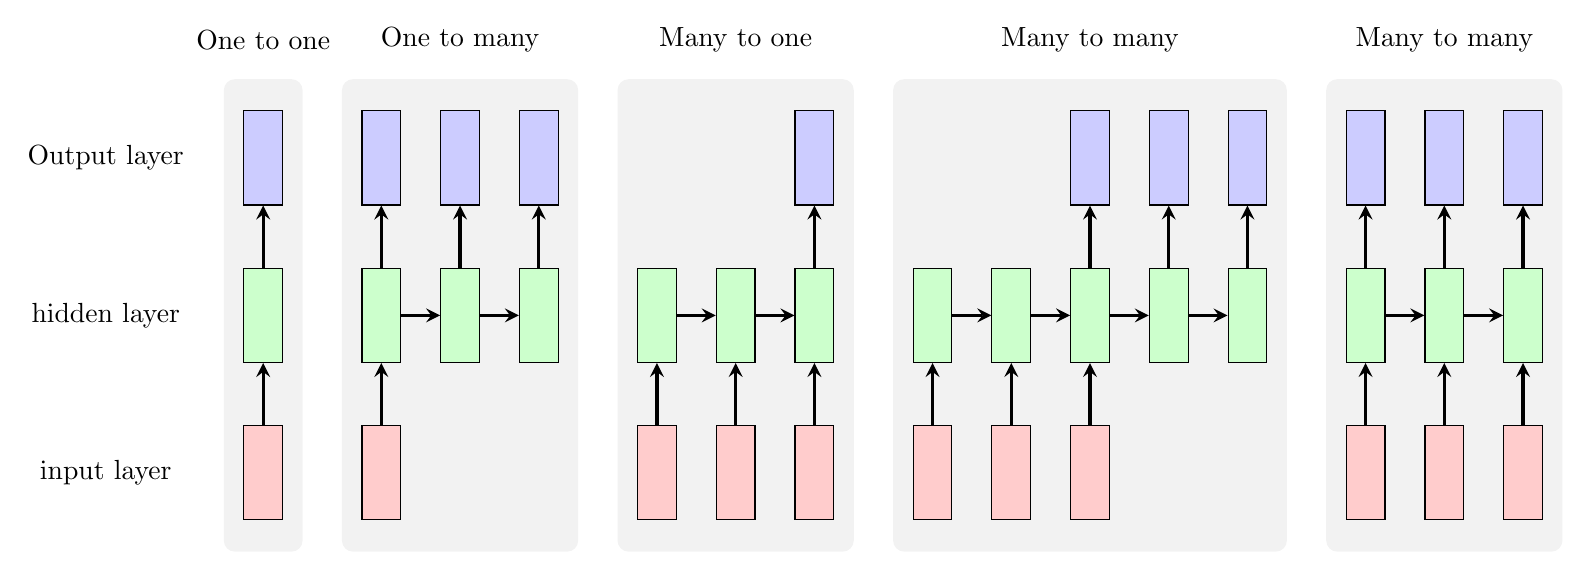
\begin{tikzpicture}
			\tikzstyle{input} = [draw,inner sep=7,minimum size=10, draw=black, fill=red!20, text width=20, text centered,rotate=90]
			\tikzstyle{hidden} = [draw,inner sep=7,minimum size=10, draw=black, fill=green!20, text width=20, text centered,rotate=90]
			\tikzstyle{output} = [draw,inner sep=7,minimum size=10, draw=black, fill=blue!20, text width=20, text centered,rotate=90]
			\tikzstyle{invisible} = [outer sep=0,inner sep=0,minimum size=0]
			\tikzstyle{stealth} = [-stealth, very thick]
			\fill [rounded corners, fill=gray!10] (-4,3.5) rectangle (-3,-2.5);
			\fill [rounded corners, fill=gray!10] (-2.5,3.5) rectangle (0.5,-2.5);
			\fill [rounded corners, fill=gray!10] (1,3.5) rectangle (4,-2.5);
			\fill [rounded corners, fill=gray!10] (4.5,3.5) rectangle (9.5,-2.5);
			\fill [rounded corners, fill=gray!10] (10,3.5) rectangle (13,-2.5);
			\node [input] (v1) at (-3.5,-1.5) {};
			\node [hidden] (v2) at (-3.5,0.5) {};
			\node [output] (v3) at (-3.5,2.5) {};
			\node [input] (v4) at (-2,-1.5) {};
			\node [hidden] (v5) at (-2,0.5) {};
			\node [hidden] (v7) at (-1,0.5) {};
			\node [hidden] (v8) at (0,0.5) {};
			\node [output] (v6) at (-2,2.5) {};
			\node [output] (v9) at (-1,2.5) {};
			\node [output] (v10) at (0,2.5) {};
			\node [input] (v11) at (1.5,-1.5) {};
			\node [input] (v13) at (2.5,-1.5) {};
			\node [input] (v15) at (3.5,-1.5) {};
			\node [hidden] (v12) at (1.5,0.5) {};
			\node [hidden] (v14) at (2.5,0.5) {};
			\node [hidden] (v16) at (3.5,0.5) {};
			\node [output] (v17) at (3.5,2.5) {};
			\node [input] (v18) at (5,-1.5) {};
			\node [input] (v20) at (6,-1.5) {};
			\node [input] (v22) at (7,-1.5) {};
			\node [hidden] (v19) at (5,0.5) {};
			\node [hidden] (v21) at (6,0.5) {};
			\node [hidden] (v23) at (7,0.5) {};
			\node [hidden] (v25) at (8,0.5) {};
			\node [hidden] (v27) at (9,0.5) {};
			\node [output] (v24) at (7,2.5) {};
			\node [output] (v26) at (8,2.5) {};
			\node [output] (v28) at (9,2.5) {};
			\node [input] (v29) at (10.5,-1.5) {};
			\node [input] (v32) at (11.5,-1.5) {};
			\node [input] (v35) at (12.5,-1.5) {};
			\node [hidden] (v30) at (10.5,0.5) {};
			\node [hidden] (v33) at (11.5,0.5) {};
			\node [hidden] (v36) at (12.5,0.5) {};
			\node [output] (v31) at (10.5,2.5) {};
			\node [output] (v34) at (11.5,2.5) {};
			\node [output] (v37) at (12.5,2.5) {};
			\draw [stealth] (v1) edge (v2);
			\draw [stealth] (v2) edge (v3);
			\draw [stealth] (v4) edge (v5);
			\draw [stealth] (v5) edge (v6);
			\draw [stealth] (v5) edge (v7);
			\draw [stealth] (v7) edge (v8);
			\draw [stealth] (v7) edge (v9);
			\draw [stealth] (v8) edge (v10);
			\draw [stealth] (v11) edge (v12);
			\draw [stealth] (v13) edge (v14);
			\draw [stealth] (v15) edge (v16);
			\draw [stealth] (v12) edge (v14);
			\draw [stealth] (v14) edge (v16);
			\draw [stealth] (v16) edge (v17);
			\draw [stealth] (v18) edge (v19);
			\draw [stealth] (v20) edge (v21);
			\draw [stealth] (v22) edge (v23);
			\draw [stealth] (v23) edge (v24);
			\draw [stealth] (v25) edge (v26);
			\draw [stealth] (v27) edge (v28);
			\draw [stealth] (v19) edge (v21);
			\draw [stealth] (v21) edge (v23);
			\draw [stealth] (v23) edge (v25);
			\draw [stealth] (v25) edge (v27);
			\draw [stealth] (v29) edge (v30);
			\draw [stealth] (v30) edge (v31);
			\draw [stealth] (v32) edge (v33);
			\draw [stealth] (v33) edge (v34);
			\draw [stealth] (v35) edge (v36);
			\draw [stealth] (v36) edge (v37);
			\draw [stealth] (v30) edge (v33);
			\draw [stealth] (v33) edge (v36);
			
			\node [invisible] at (-3.5,4) {One to one};
			\node [invisible] at (-1,4) {One to many};
			\node [invisible] at (2.5,4) {Many to one};
			\node [invisible] at (7,4) {Many to many};
			\node [invisible] at (11.5,4) {Many to many};
			\node [invisible] at (-5.5,-1.5) {input layer};
			\node [invisible] at (-5.5,0.5) {hidden layer};
			\node [invisible] at (-5.5,2.5) {Output layer};
			\end{tikzpicture}
		}      
		\caption{Arquitecturas de modelo}%\cite{karpathy}.
		\label{fig: model_archs}
	\end{figure}
\end{frame}
\begin{frame}[fragile]{Diseño e implementación de modelos.\newline Modelo de capas LSTM II}
\begin{lstlisting}[basicstyle=\tiny\ttfamily, caption={Resumen del modelo},captionpos=b, label={lst: model_resume},frame=none, xleftmargin=.2\textwidth]
_________________________________________________________________
Layer (type)                 Output Shape              Param #   
=================================================================
lstm (LSTM)                  (None, 1, 512)            1562624   
_________________________________________________________________
lstm_1 (LSTM)                (None, 1, 512)            2099200   
_________________________________________________________________
lstm_2 (LSTM)                (None, 512)               2099200   
_________________________________________________________________
dense (Dense)                (None, 250)               128250    
=================================================================
Total params: 5,889,274
Trainable params: 5,889,274
Non-trainable params: 0
_________________________________________________________________
\end{lstlisting}
\end{frame}
\begin{frame}[fragile]{Diseño e implementación de modelos.\newline Modelo de capas LSTM III}
	\vspace*{5pt}
	Debido al gran número de datos, \textbf{294 Gbytes}, se debe entrenar con un generador de secuencias, además los datos van a ser normalizados
	\begin{figure}
		\centering
		\begin{subfigure}[t]{0.4\textwidth}
			\centering
			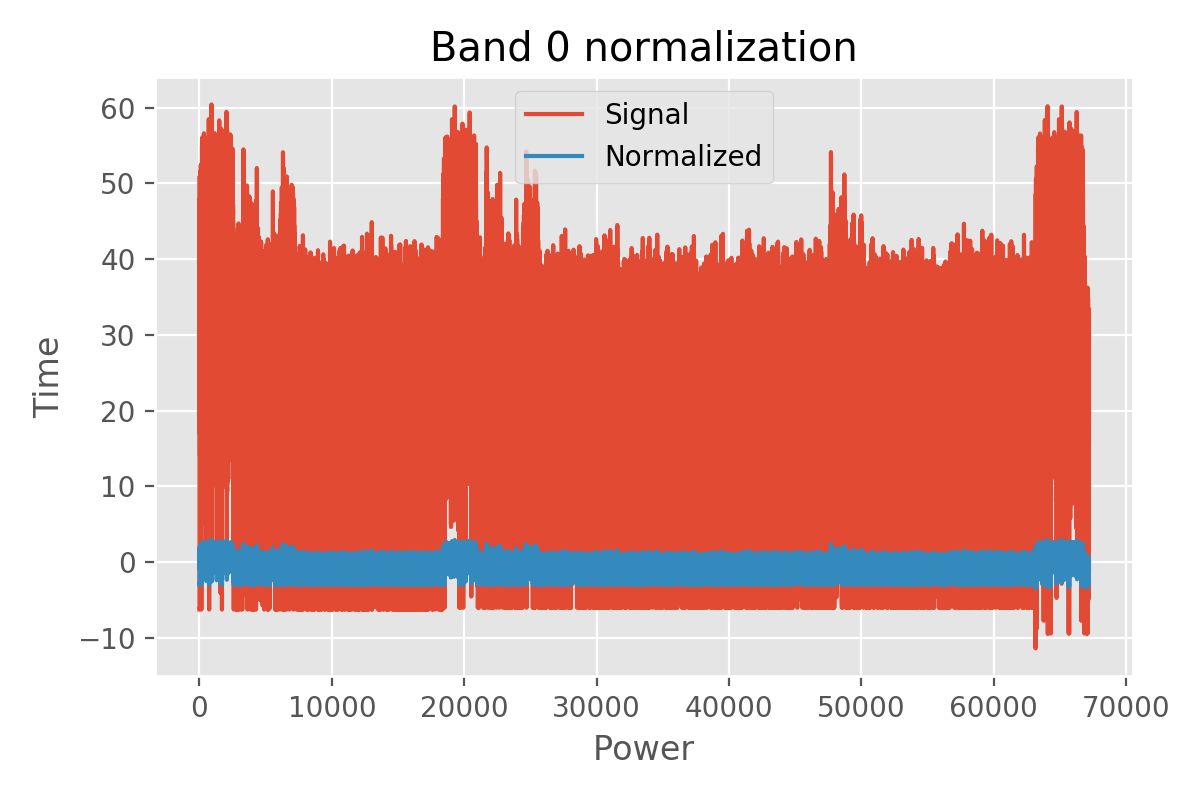
\includegraphics[width=\columnwidth]{../figures/band0_norm}
			\vspace*{-7pt}
			\caption{Comparación de la señal con su normalización en tiempo para la banda cero de un mismo audio con ruido}
			\label{fig: norm_time}
		\end{subfigure}%
		\hspace*{10pt}
		\begin{subfigure}[t]{0.4\textwidth}
			\centering
			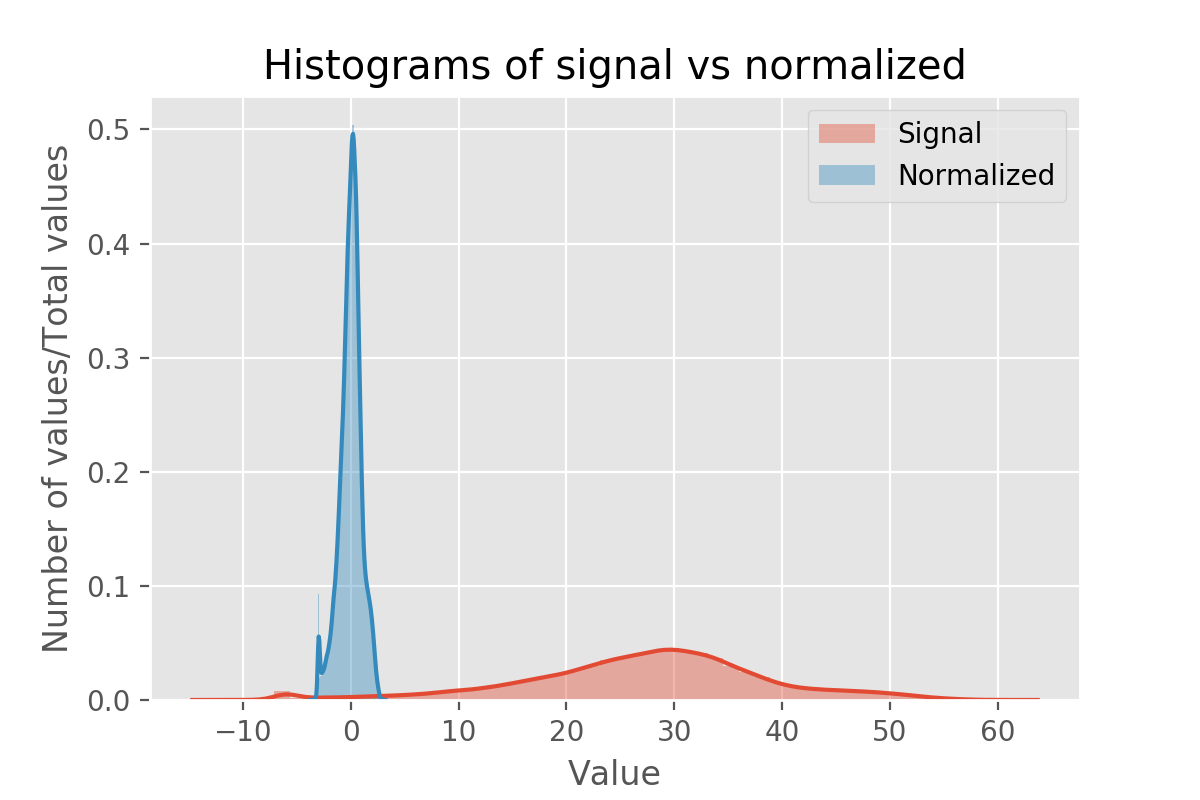
\includegraphics[width=\columnwidth]{../figures/band0_norm_hist}
			\vspace*{-7pt}
			\caption{Comparación de los histogramas de la señal y su normalización para la banda cero de un mismo audio con ruido}
			\label{fig: norm_hist}
		\end{subfigure}
	\end{figure}
	\vspace*{-17pt}
	\begin{figure}
		\centering
		\begin{subfigure}[t]{0.4\textwidth}
			\centering
			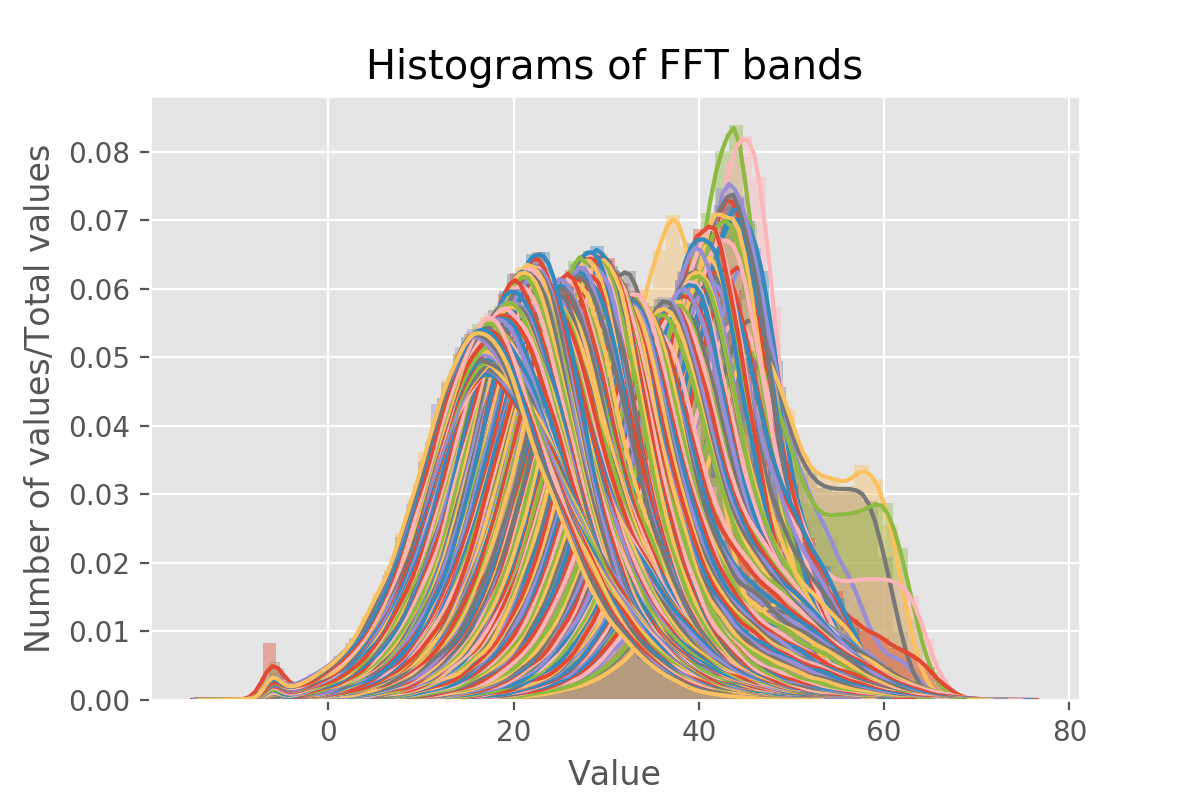
\includegraphics[width=\textwidth]{../figures/bands_hist}
			\vspace*{-7pt}
			\caption{Histograma de todas las bandas}
			\label{fig: bands_hist}
		\end{subfigure}%
		\hspace*{10pt}
		\begin{subfigure}[t]{0.4\textwidth}
			\centering
			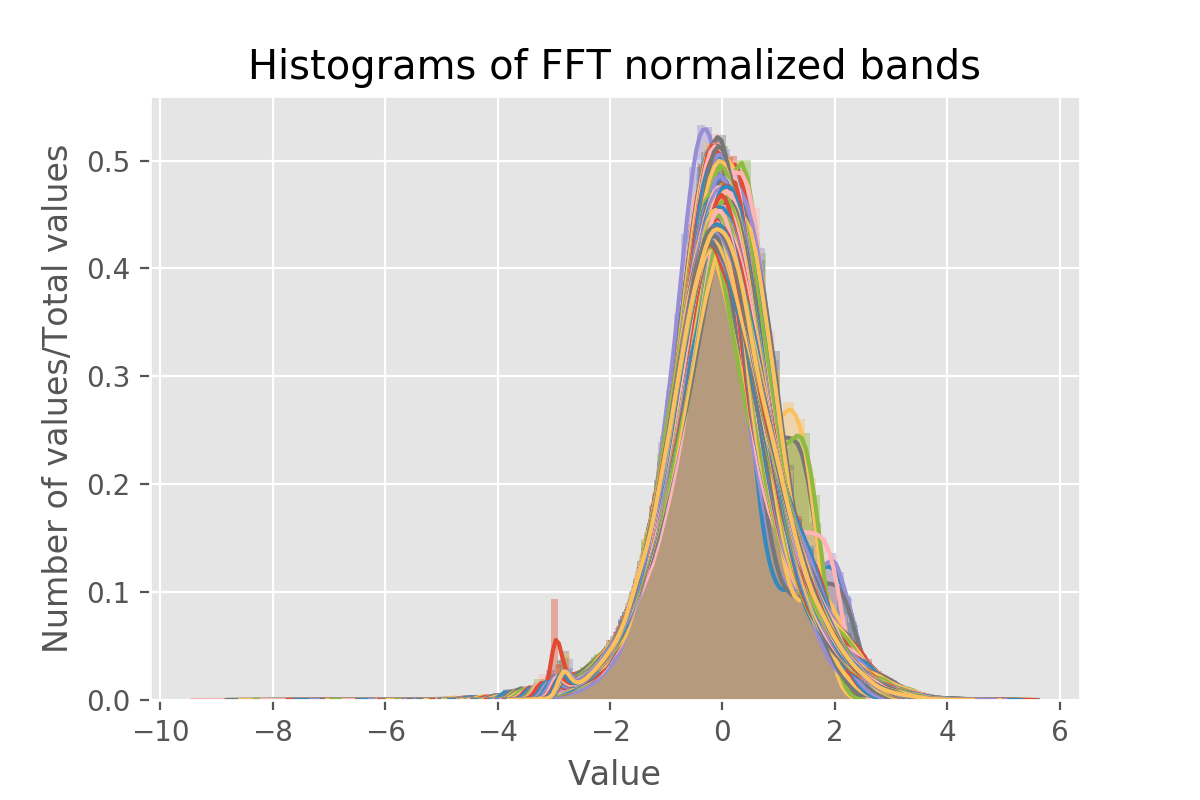
\includegraphics[width=\textwidth]{../figures/bands_norm_hist}
			\vspace*{-7pt}
			\caption{Histograma de todas las bandas normallizadas}
			\label{fig: bands_norm_hist}
		\end{subfigure}
	\end{figure}
\end{frame}